\documentclass[17pt,a4paper,landscape]{extarticle}
\usepackage[margin=1.45cm,top=0.45cm,bottom=0.7cm,left=0.9cm,right=0.9cm]{geometry}
\usepackage{amsmath}
\usepackage{amssymb}
\usepackage{tasks}
\usepackage{graphicx}
\usepackage{xcolor}
\usepackage[sfdefault,lf]{FiraSans}
\renewcommand{\familydefault}{\sfdefault}
\setlength{\parindent}{0pt}
\pagestyle{empty}
\settasks{label=\textbf{\arabic*.}, label-width=2.2em, item-indent=2.95em, column-sep=1.2cm, after-item-skip=1.2em}
\everymath{\displaystyle}

\begin{document}
\sffamily
\boldmath

{\LARGE \textbf{Drawing straight-line from given equation — Foundation}}\\[0.2em]
Plot a few points, then draw the full line.

\begin{tasks}(3)
\task {Draw $y=x+1$. \\[0.4em] 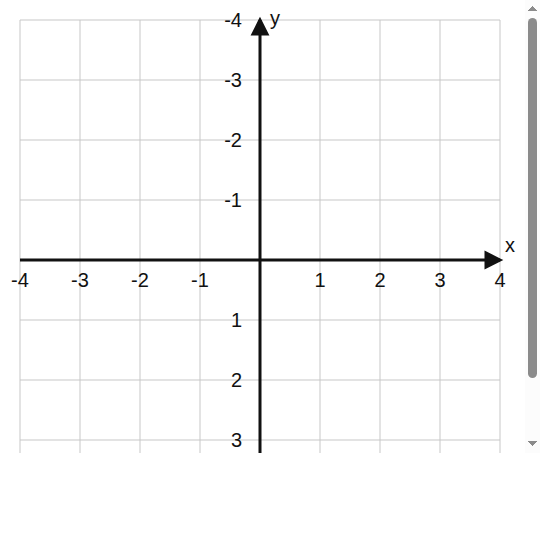
\includegraphics[width=0.88\linewidth]{web-diagrams/coord-grid.png}}
\task {Draw $y=x-2$. \\[0.4em] 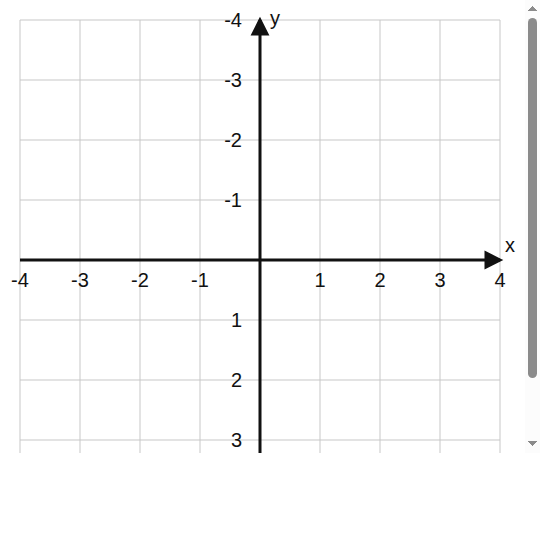
\includegraphics[width=0.88\linewidth]{web-diagrams/coord-grid.png}}
\task {Draw $y=2x$. \\[0.4em] 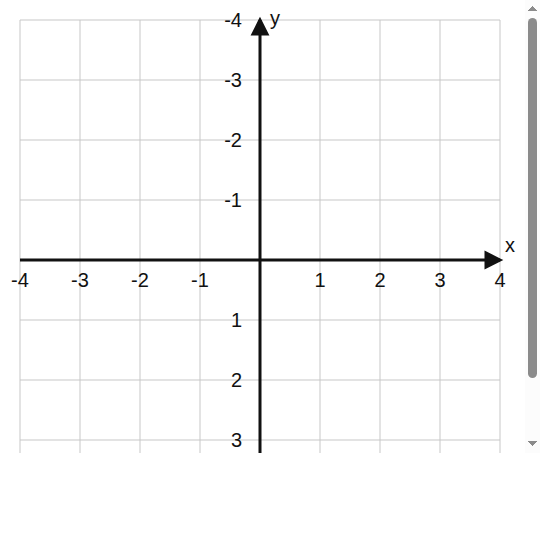
\includegraphics[width=0.88\linewidth]{web-diagrams/coord-grid.png}}
\task {Draw $y=2x+1$. \\[0.4em] 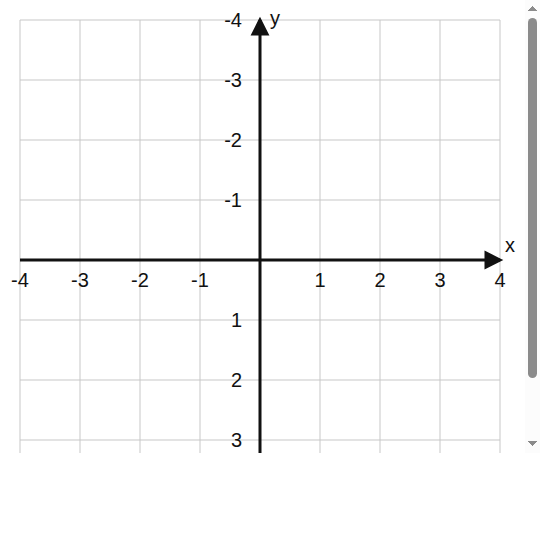
\includegraphics[width=0.88\linewidth]{web-diagrams/coord-grid.png}}
\task {Draw $y=-x+3$. \\[0.4em] 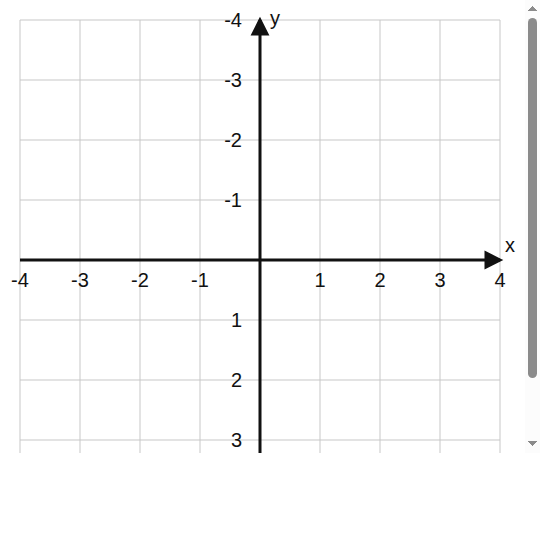
\includegraphics[width=0.88\linewidth]{web-diagrams/coord-grid.png}}
\task {Draw $y=-x-1$. \\[0.4em] 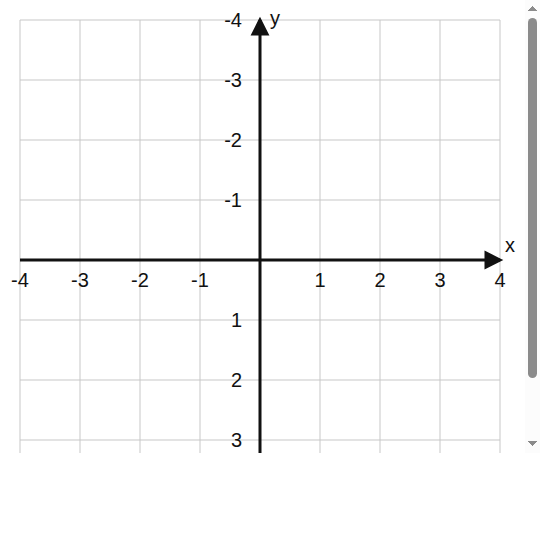
\includegraphics[width=0.88\linewidth]{web-diagrams/coord-grid.png}}
\task {Draw $y=3x-2$. \\[0.4em] 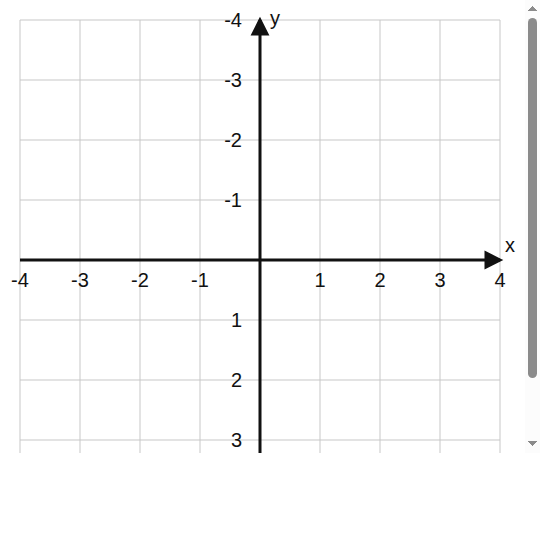
\includegraphics[width=0.88\linewidth]{web-diagrams/coord-grid.png}}
\task {Draw $y=-2x+2$. \\[0.4em] 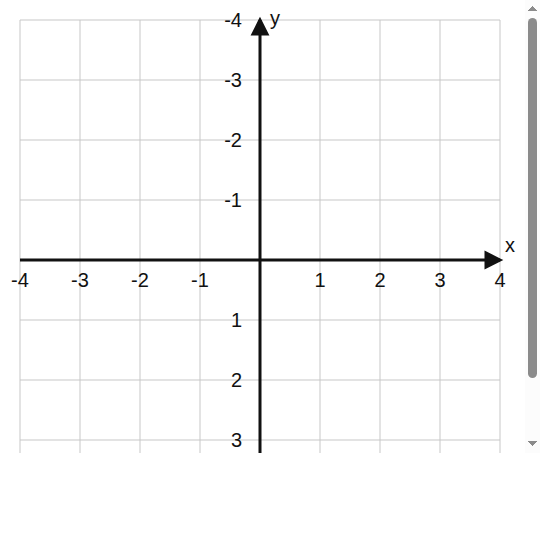
\includegraphics[width=0.88\linewidth]{web-diagrams/coord-grid.png}}
\task {Draw $y=\frac{1}{2}x+1$. \\[0.4em] 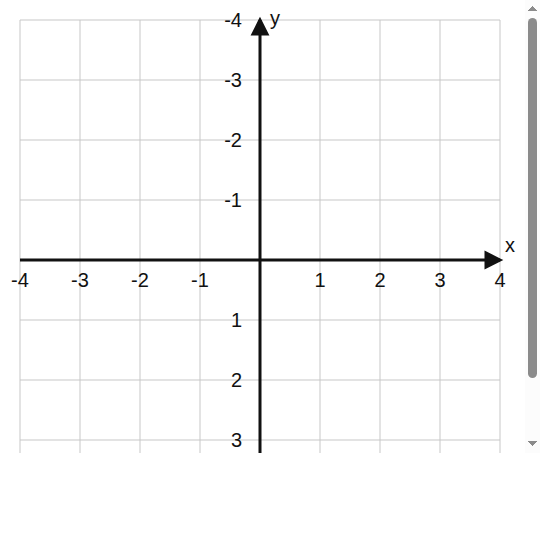
\includegraphics[width=0.88\linewidth]{web-diagrams/coord-grid.png}}
\task {Draw $y=\frac{1}{2}x-2$. \\[0.4em] 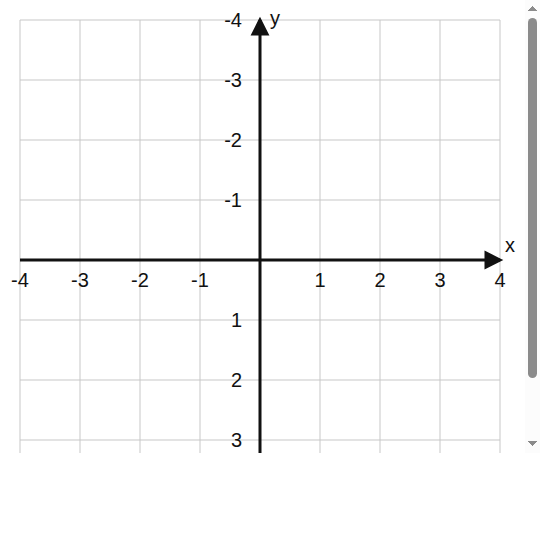
\includegraphics[width=0.88\linewidth]{web-diagrams/coord-grid.png}}
\task {Draw $y=-\frac{1}{2}x+2$. \\[0.4em] 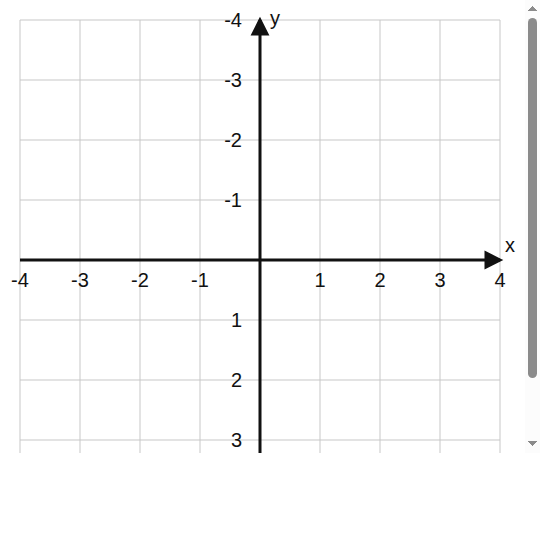
\includegraphics[width=0.88\linewidth]{web-diagrams/coord-grid.png}}
\task {Draw $y=-\frac{1}{2}x-1$. \\[0.4em] 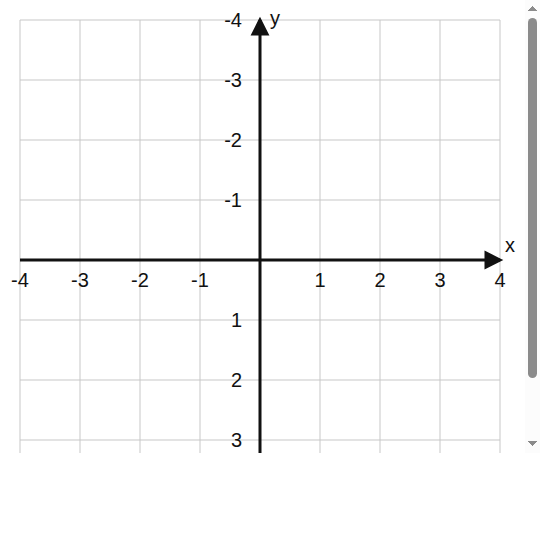
\includegraphics[width=0.88\linewidth]{web-diagrams/coord-grid.png}}
\end{tasks}

\end{document}
